% !TEX root = main.tex

\section{Introduction}\label{sec:intro}

Indoor person localization is still a challenge that needs to be faced to make this technology usable in various situtation as location-based life improving services, firefighters localization and navigation, patients tracking 
motion monitoring, medical observation or accident monitoring \cite{pourhomayoun2012spatial}.
A common way to localize a body in space is to use odometry information that can be processed from data captured by plenty of sensors, from GPS to cameras.
The quality of this information is also known to be dependent on the sensor's specifications and to accumulate measurement errors during integration. 
SLAM (Simultaneous Localization And Mapping) handles this problem with loop closure strategies correcting the pose of a body and thus reducing the effects of imperfect sensors.

\cite{hutchings1998system} introduced the idea of person localization using a foot-mounted IMU in 1997. Since then, many developments have been made to find alternative ways to accurately localize people.
Pedestrian Dead Reckoning (PDR) methods, also known as Personal Navigation Devices, make use of one or more Inertial Measurement Units (IMU) installed on the subject's body.
The main idea of PDR techniques is to integrate IMU's measurements with Zero Velocity Update constraints to reduce errors \cite{ojeda2007personal}.
This work is extensively used in IMU-based human localization works and various fields. \cite{kwanmuang2015phd} analyses the gait of a walking person 
with PDR method to estimate the direction of the shoe, thus the walking direction, and measure stride lenght. \cite{jin2011robust} uses multiple dead-reckoning systems on a single human 
agent and constraints on relative displacements of each system to others with respect to the center of motion to create a tracking system
greatly reducing errors when compared to a traditional dead-reckoning method. As we can see, shoe-mounted IMU is still considered as a possible way to
accurately localize persons in an indoor environment. One way to understand why foot-mounted IMU is prefered to other alternatives may be given by \cite{groves2007inertial} 
comparing body-mounted and foot-mounted based PDR methods. 
Both systems had similar performances considering the position error, being lower than 10 m for 60 seconds experiments. However, the foot-mounted shown drifts as results were compared
to GPS ground truth. We should note that the body-mounted method proved to be usable in not only walking cases but also when the human agent was jogging or running but with a decrease in terms of accuracy.

Various strategies can be considered to improve the localization results of foot-mounted IMU navigation.To achieve this goal, one way to consider is the use of one or more IMU and define some special constraints.
The main advantage of this choice is that the solution would be easily wearable and thus usable.
As shown in \cite{kourogi2010method} and \cite{panahandeh2012chest}, PDR can be used to recognize the action being carried out by the pedestrian through classification methods, but adding this contextual 
information is also a way to reduce PDR localization errors (\cite{kourogi2010method}). \cite{wagstaff2017improving} is not only using this contextual information 
thanks to a the training of a support vector machine (SVM) classifier using IMU data, but also doing efforts on finding optimal zero-velocity detection parameters taking into account 
a specific user and motion types. 
One other possibility that can be considered is to limit the drift of one IMU with other units placed in other places of the body. Skog et al. successfully limited the position error
of a dual foot-mounted IMUs system composed of an IMU on each foot and the use of inequality constraints \cite{skog2012fusing}. In that case, the additive constraint was related to the maximum step length the pedestrian could do.
Thus the inequality constraints limit the distance between both IMUs to give better position estimation results when compared to sinle foot-mounted IMU solution.

Fusion strategies with information coming from different sensors can also be used to impprove localization results as it is already done
for in robotics. At this end we could use GPS information (\cite{sukkarieh1999high,hide2012investigating,gao2014data}), received signal stregth indicator (RSSI) from wireless communication as considered
in \cite{malyavej2013indoor} using wireless local area networks (WLAN) or radio-frequency identification (RFID) tags placed at known locations in \cite{ruiz2012accurate}
along with other drift reduction methods such as zero velocity updates (ZUPTs), zero angular-rate updates (ZARU) and the use of magnometers.
Using these strategies is presented by \cite{ruiz2012accurate} as a successfull solution to overcome the drift observed in methods using IMU and to obtain positionning errors of approximately 1.5 m.
Chdid et al. in \cite{chdid2011inertial} are using a foot-mounted IMU fused with a waist-mounted visual odometry system to update the state of the system composed of its position, velocity and acceleration.
This last system was used recently by Pierce et al. \cite{pierce2016incorporation} to design a fusion strategy requiring measurements only once per human step instead of every time step.

Angermann et al. applied a SLAM approach to pedestrian localization using foot-mounted IMU and human perception in indoor environment \cite{angermann2012footslam}. Experiments show that
FootSLAM is able to bound the error growth to 1 meter through the use of dynamic bayesian network (DBN) formulation of the problem and loop closure strategies. The idea exploited here is to use the normal human behavior 
consisting on relying on visual information to guide the motion and avoid obstacles. FootSLAM's idea gave birth to several variants for use in different conditions or slightly different purposes (\cite{puyol2012complexity,bruno2011wislam}).
Hardegger et al. use contextual information to body-mounted IMUs with a FastSLAM-base implementationin ActionSLAM, landmarks being location-related actions \cite{hardegger2012actionslam}. 
A foot-mounted IMU is then used not only for inertial navigation purposes but also as a landmark observation system through action recognition strategies by applying machine learning techniques for motion classification.
The main idea behing ActionSLAM is to consider that some specific actions are done only at some specific locations on the map. Results tend to show that using both foot-mounted and wrist-mounted IMUs
is giving results that are robust enough for indoor applications.

Previously cited example tend to show how important it is for pedestrian inertial navigation system to be able to deal with the localization drifts due to the integration of IMU's data.

\TODO{Add cover figure}
% \begin{figure}
% \centering
% 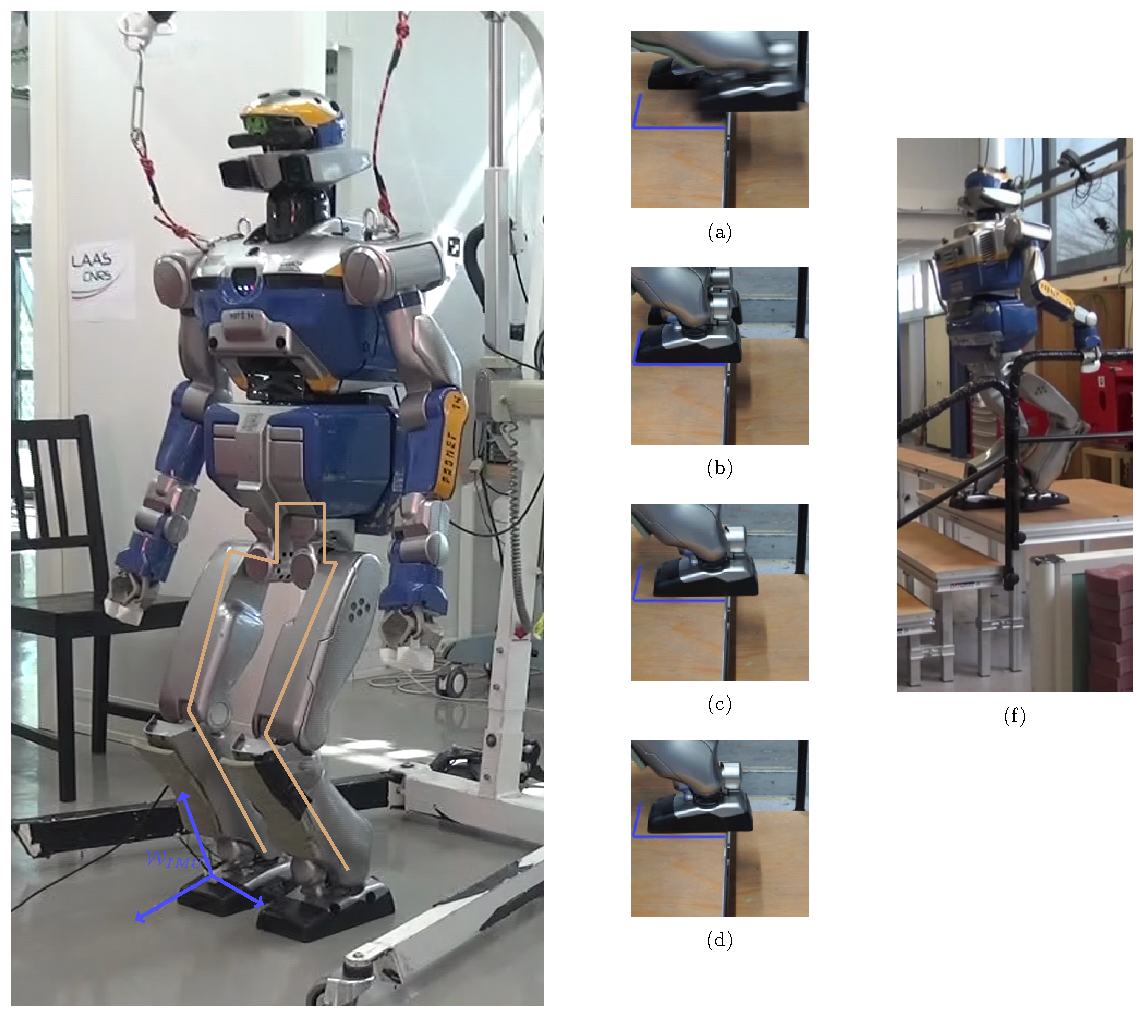
\includegraphics[width=\linewidth]{./figures/cover-figure.pdf}
% 	\caption{D(from \cite{Carpentier:ICRA:2016}).
%  }
% 	\label{fig:cover}
% \end{figure}


Graphical methods have been extensively used to implement such fusion strategies \cite{Thrun:ijrr:2006,Kaess:itro:2008}.
They have been used for large modeling estimation problems by means of sparse networks of constraints. 
In robotics, the problems of visual odometry, and simultaneous localization and mapping, have reached a high degree of maturity, 
in great part thanks of the graphical representation. 
This is so, among other aspects, because of the power of the graphical representation to accurately model complex estimation problems. 
These often involve dynamics, proprioceptive measures, exteroceptive measures, and self-calibration.
The graphical representation also allows for the design of powerful nonlinear estimation solvers, which can be built taking into account the needs for accuracy, 
robustness and CPU-performance.
In order to keep the problem tractable and maintain real-time performance a key point is to avoid the graph to be too large for a given time window.
IMUs are challenging in this regards, as their high frequency measurements create large sets of data. 
 
For this reason, \cite{LUPTON-09,forster2015imu} proposed to pre-integrate the IMU information over an horizon where IMU data are the only
ones to be measured.
A first contribution of this paper is to reformulate the method proposed in \cite{forster2015imu} from rotation matrix to quaternion representation
and give a detailed and simpler algebraic derivation.
The second contribution is to apply this method to the measurement of a humanoid robot flying foot pose.
The level of accuracy obtained with this approach allows us to detect foot slippage. 
Finally, we describe the implementation of this pre-integration scheme in a software implementation of the graphical method.





